\section{通道\channel }
\begin{frame}{用途和种类}
    \begin{itemize}
        \item \textbf{用途}: 以线程安全的方式实现不同协程之间的通信 
        \item 通道在声明时指定其数据流向
            \begin{itemize}
                \item \alert{读写}\quad 默认,例如,\code{xStream := make(chan int)}
                \item \alert{只读}\quad 将<-箭头放在\code{chan}关键字的左边,例如,\code{yStream := make(<-chan int)}
                \item \alert{只写}\quad 将<-箭头放在\code{chan}关键字的右边,例如,\code{zStream := make(chan<- int)}
            \end{itemize}
    \end{itemize}

    \begin{exampleblock}{温馨提示}
        go 会在必要时隐式地将单向通道(只读/只写)转为双向通道(读写) 
    \end{exampleblock}
\end{frame}

\begin{frame}[fragile]{数据类型与传递}
    \begin{itemize}
        \item 通道传递的数据类型可以被指定
        \item 对于一个可读通道\code{c},可以利用表达式\code{c <- x}将值\code{x}放到通道里
        \item 对于一个可写通道\code{c},可以利用表达式\code{y <- c}从通道里取出值\code{y}
    \end{itemize}
\begin{lstlisting}[caption={通道数据传递样例}]
stringStream := make(chan string)
go func() {
  stringStream <- "Hello channels!"
}()
fmt.Println(<-stringStream)

// 输出:
// Hello channels!    
\end{lstlisting}    
\end{frame}

\begin{frame}[fragile]{导致编译错误的操作}
\begin{itemize}
    \item 对只读通道的写操作
\begin{lstlisting}
readStream := make(<- chan interface{})
readStream <- struct{}{}

// 输出:
// invalid operation: readStream <- struct {} literal 
// (send // to receive-only type <-chan interface {})    
\end{lstlisting}
        \item 对只写通道的读操作
\begin{lstlisting}
writeStream := make(chan<- interface{})
<- writeStream

// 输出:
// invalid operation: <-writeStream (receive from 
// send-only type chan<- interface {})
\end{lstlisting}
\end{itemize}
\end{frame}

\begin{frame}{阻塞性}
    \begin{itemize}
        \item 任何尝试向容量已满的通道发送数据的协程会等待直至通道有剩余空间
        \item 任何尝试向空通道读数据的协程都会等待直至有一个值进入通道
    \end{itemize}
\end{frame}

\begin{frame}[fragile]{读操作的两种方式}
    \begin{itemize}
        \item 只返回一个值: 从通道传输下来的数值
        \item 返回一个值\code{x}和一个布尔值\code{closed}
            \begin{itemize}
                \item \code{x}表示从通道传输下来的数据
                \item \code{closed=false}表示\code{x}是由于通道已关闭其容量为空而返回的所声明类型的默认值
                \item \code{closed=false}则表示\code{x}是从别处写入通道的值
            \end{itemize}
    \end{itemize}

\begin{lstlisting}[caption={通道的两种读取操作}]
stringStream := make(chan string)
go func() {
  stringStream <- "Hello channels!"
}()

salutation, ok := <-stringStream
fmt.Printf("(%v): %v", ok, salutation)

// 输出:
// (true): Hello channels!
\end{lstlisting}
\end{frame}

\begin{frame}{通道的关闭}
    \begin{itemize}
        \item \code{close(c)}函数调用可关闭通道\code{c}
        \item 可读通道能够满足无限的读请求(即使通道已被关闭)
    \end{itemize}
\end{frame}

\begin{frame}[fragile]{设计模式1: \code{for...range}遍历}
    \code{range}和\code{for}关键字组合可以通道作为实参,并在通道关闭时自动跳出循环
\begin{lstlisting}
intStream := make(chan int)

go func() {
    defer close(intStream)
    for i := 1; i <= 5; i++ {
    intStream <- i
    }
}()

for integer := range intStream {
    fmt.Printf("%v ", integer)
}

// 输出:
// 1 2 3 4 5 
\end{lstlisting}    
\end{frame}

\begin{frame}[fragile]{设计模式2: 作为取消信号}
    以通道的关闭为信号通知多个协程
\begin{lstlisting}
begin := make(chan interface{})
var wg sync.WaitGroup
for i := 0; i < 3; i++ {
    wg.Add(1)
    go func(i int) {
        defer wg.Done()
        <-begin
        fmt.Printf("%v has begun\n", i)
    }(i)
}
fmt.Println("Unblocking goroutines...")
close(begin)
wg.Wait()

// Unblocking goroutines...
// 1 has begun
// 0 has begun
// 2 has begun
\end{lstlisting}
\end{frame}

\begin{frame}{容量}
    \begin{itemize}
        \item 通道根据容量可划分为 2 种类型:\alert{非缓存型}和\alert{缓存型}
        \item 非缓存型: 声明时不指定容量或指定容量为 0
        \item 缓存型: 通道在初始化时被赋予大于 0 的容量
            \begin{itemize}
                \item 给定容量为\code{n},对通道\code{c}可同时支持\code{n}个写操作
                \item 可作为一个内存型消息队列实现并发进程间的通信
                \item 通道为空且有挂起的等待协程时,新值的传入会绕过通道直接传给等待协程
                \item 这类通道容易\alert{导致过早优化问题}和\alert{隐藏死锁问题}
            \end{itemize}
    \end{itemize}
    通道的满和空都是相对与通道的容量而言的 


    在预知通道需要支持的并发写操作次数\code{n}时,容量大小为\code{n}的缓存型通道可以使得写操作尽可能快地执行,例如,\href{https://github.com/sammyne/concurrency-in-go/blob/master/chapter03/channels/buffered_channel.go}{缓存型通道作为消息队列}
\end{frame}

\begin{frame}[fragile]{\texttt{nil}通道}
    给定\code{nil}通道\code{c}
    \begin{itemize}
        \item 对\code{c}的读操作会阻塞进程(尽管并不一定会导致死锁??)
\begin{lstlisting}
    fatal error: all goroutines are asleep - deadlock!
\end{lstlisting}
        \item 对\code{c}的写操作也会阻塞进程
\begin{lstlisting}
fatal error: all goroutines are asleep - deadlock!
\end{lstlisting}
        \item 关闭\code{c}会触发\code{panic}
\begin{lstlisting}
    panic: close of nil channel 
\end{lstlisting}
    \end{itemize}
\end{frame}

\begin{frame}{对通道不同操作的后果}

\begin{figure}
    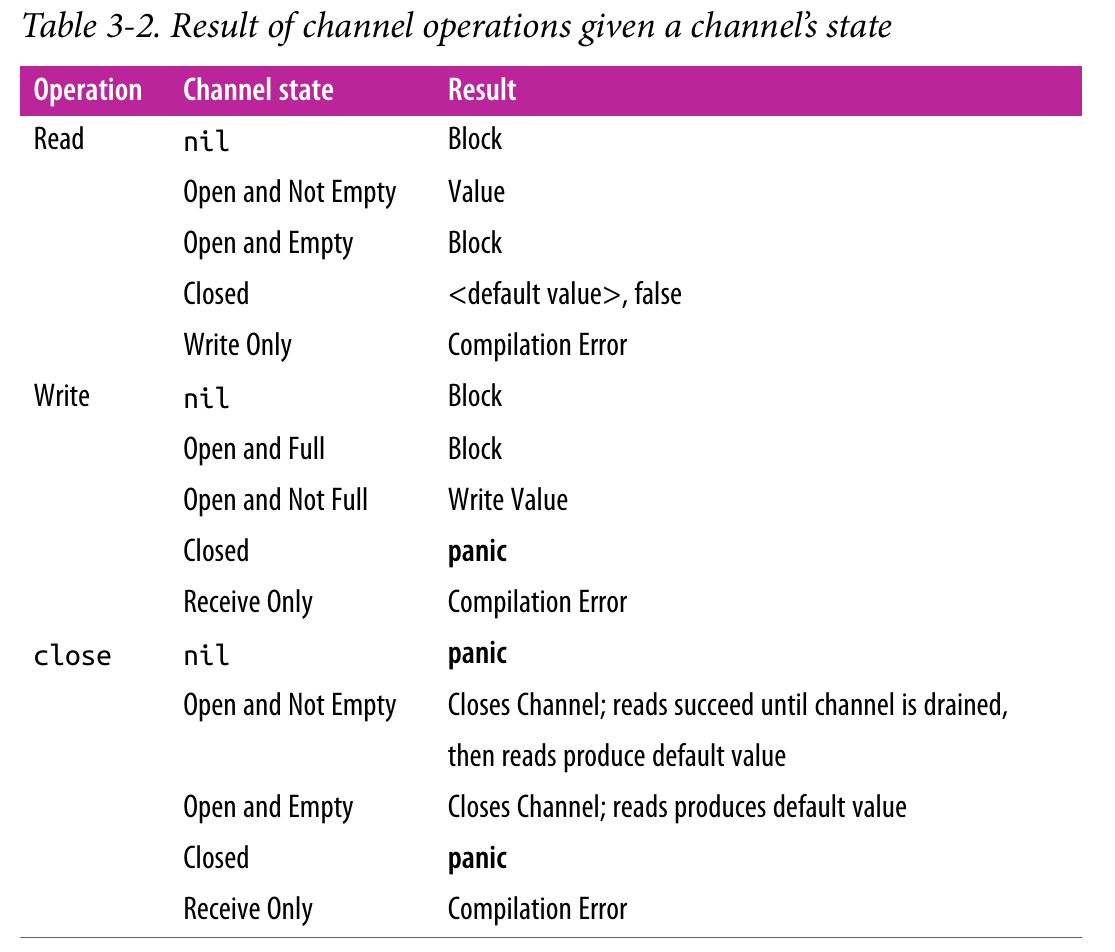
\includegraphics[width=0.5\textwidth]{images/channel-operations.png}
    \caption{对通道不同操作的后果}
\end{figure}

    由表可知,
\begin{itemize}
    \item 阻塞协程的操作有 3 种
    \item 导致协程恐慌的操作有 3 种
\end{itemize}
\end{frame}

\begin{frame}{上下文}
    通道的正确使用需要有合理的上下文环境,而为通道赋予正确的所有权协助创造这种环境

    \alert{通道的所有权应该属于负责初始化、写入数据和关闭通道的协程}
    
    通过这种规则限定
    \begin{itemize}
        \item \alert{所有者}持有对通道的\alert{读写权限},并负责
            \begin{itemize}
                \item 初始化通道
                \item 执行写操作或将通道所有权转移给其他协程
                \item \alert{关闭通道}
                \item 将以上 3 项封装为一个只读通道暴露给消费者
            \end{itemize}
        \item \alert{消费者}则对通道只有\alert{读权限},只需关心
            \begin{itemize}
                \item 监听通道的关闭
                \item 负责处理任何情况下的阻塞
            \end{itemize}
    \end{itemize} 
\end{frame}

\begin{frame}[fragile]{基于通道实现的所有者---消费者样例}
    \begin{columns}[t]
        \column{0.65\textwidth}
\begin{lstlisting}[xleftmargin=8pt]
chanOwner := func() <-chan int {
    resultStream := make(chan int, 5)
    go func() {
        defer close(resultStream)
        for i := 0; i <= 5; i++ {
        resultStream <- i
        }
    }()
    return resultStream
}
    
resultStream := chanOwner()
for result := range resultStream {
    fmt.Println("Received:", result)
}
fmt.Println("Done!")

\end{lstlisting}
        \column{0.3\textwidth}
\begin{lstlisting}[firstnumber=last,xleftmargin=8pt]
// 输出:
// Received: 0
// Received: 1
// Received: 2
// Received: 3
// Received: 4
// Received: 5
// Done!    
\end{lstlisting}
    \end{columns}
\end{frame}